\subsection{Relación con la Estimación}
\label{subsec:relacion}

\textbf{Estimación vs Calendarización:}

\begin{table}[h]
    \centering
    \begin{tabularx}{\textwidth}{|l|X|X|}
        \hline
        \textbf{Aspecto} & \textbf{Estimación}             & \textbf{Calendarización}      \\
        \hline
        Propósito        & Calcular esfuerzo/tiempo        & Fijar fechas y paralelización \\
        \hline
        Paralelismo      & No considera tareas simultáneas & Gestiona dependencias         \\
        \hline
        Entregas         & Sin fechas específicas          & Establece hitos y entregas    \\
        \hline
        Ejemplo:          & ``Requiere 40 personas-mes''    & ``Versión 1.0 para 15/Oct''   \\
        \hline
    \end{tabularx}
    \label{tab:comparacion-estimacion-calendarizacion}
\end{table}

\subsection{Dificultades Comunes}
\label{subsec:dificultades}

\begin{enumerate}
    \item Fechas límite \textbf{irreales} impuestas externamente
    \item \textbf{Cambios constantes} en requisitos del cliente
    \item \textbf{Subestimación} de esfuerzo/recursos
    \item \textbf{Riesgos no considerados} inicialmente
    \item Problemas técnicos \textbf{imprevistos}
    \item \textbf{Falta de comunicación} en el equipo
    \item Negación de \textbf{retrasos} y correcciones
\end{enumerate}

\subsection{Manejo de Fechas Límite}
\label{subsec:fechas}

\textbf{Estrategias efectivas:}

\begin{itemize}
    \item \textbf{Estimación detallada:} Usar datos históricos de proyectos similares
    \item \textbf{Desarrollo incremental:}
    \begin{itemize}
        \item Establecer qué funcionalidad corresponde a cada entrega
        \item Asegurar las funcionalidades mínimas básicas antes de cada entrega
    \end{itemize}
    \item \textbf{Comunicación proactiva:}
    \begin{enumerate}
        \item Demostrar con datos por qué la fecha es irreal
        \item Proponer alternativas concretas
        \item Negociar alcance vs.\ tiempo
    \end{enumerate}
    \item \textbf{Enfoque ágil:}
    \begin{itemize}
        \item \textbf{Sprints} cortos con entregables concretos
        \item \textbf{Priorización flexible} con el cliente
    \end{itemize}
\end{itemize}

\subsection{Hitos y Entregas}
\label{subsec:hitos}

\begin{itemize}
    \item \textbf{Hito válido:}
    \begin{itemize}
        \item Final de etapa lógica (ejemplo: \textquote{Prototipo móvil terminado})
        \item Medible y verificable
        \item Responsable asignado
    \end{itemize}
    \item \textbf{Anti-ejemplo:}
    \begin{itemize}
        \item \textquote{50\% del código funciona} (no verificable)
    \end{itemize}
    \item \textbf{Entrega:}
    \begin{itemize}
        \item Hito entregado al cliente
        \item Ejemplo: \textquote{Versión con registro de usuarios}
        \item Debe incluir criterios de aceptación claros
    \end{itemize}
\end{itemize}

\subsection{Dependencias entre Tareas}
\label{subsec:dependencias}
\deactivatequoting
\begin{center}
    \begin{tabularx}{\textwidth}{|l|l|X|c|}
        \hline
        \textbf{Tipo} & \textbf{Notación} & \textbf{Descripción}                                                             \\
        \hline
        Fin-Inicio    & FS                & B no empieza hasta que A termina (\textit{ejemplo: Pruebas después de desarrollo})    \\
        \hline
        Inicio-Inicio & SS                & B no empieza hasta que A empieza (\textit{ejemplo: Diseño UI y \textquote{back-end}}) \\
        \hline
        Fin-Fin       & FF                & B no termina hasta que A termina (\textit{ejemplo: Documentación y codificación})     \\
        \hline
        Inicio-Fin & SF & B no termina hasta que A empieza (\textit{rara en software})
        \\
        \hline
    \end{tabularx}
\end{center}
\activatequoting

\textbf{Ejemplos prácticos:}

\begin{itemize}
    \item \textbf{FS:} Pruebas no pueden comenzar hasta que desarrollo termine
    \item \textbf{SS:} Diseño UI y diseño DB pueden comenzar simultáneamente
    \item \textbf{FF:} Documentación no puede completarse hasta que desarrollo finalice
    \item \textbf{SF:} Mantenimiento no puede terminar hasta que despliegue comience
\end{itemize}

\subsection{Diagrama de Gantt}
\label{subsec:gantt}
Se muestra el diagrama de Gantt en la \autoref{fig:diagrama-gantt}.
\begin{itemize}
    \item \textbf{Elementos clave:}
    \begin{itemize}
        \item Tareas en eje vertical
        \item Tiempo en eje horizontal
        \item Barras horizontales = duración
    \end{itemize}
    \item \textbf{Ventajas:}
    \begin{itemize}
        \item Visualización clara del cronograma
        \item Identificación de solapamientos
        \item Seguimiento de progreso
    \end{itemize}
    \item \textbf{Ejemplo:}
    \begin{figure}[h]
        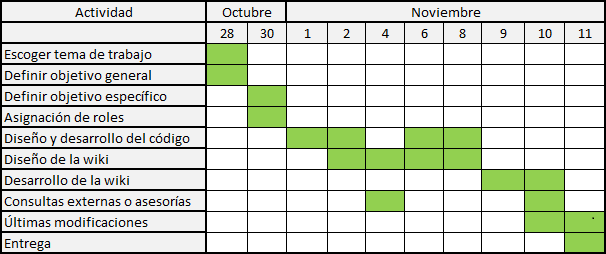
\includegraphics[width=0.75\textwidth]{imagenes/gantt_ejemplo}
        \caption{Diagrama de Gantt}
        \label{fig:diagrama-gantt}
    \end{figure}
\end{itemize}

\subsection{Diagrama de PERT}
\label{subsec:pert}

Proporciona una representación visual del cronograma de un proyecto y desglosa las tareas individuales.

\subsubsection{Conceptos fundamentales}

\begin{itemize}
    \item \textbf{Nodos:} Representan eventos (no actividades)
    \item \textbf{Flechas:} Actividades con duración
    \item \textbf{Camino crítico:} Ruta más larga (determina duración total)
\end{itemize}

\subsubsection{Elementos}

Este diagrama tiene los elementos de la \autoref{tab:tabladiapert}.

\begin{table}[htbp]
    \centering
    \begin{tabularx}{\textwidth}{|l|X|}
        \hline
        \textbf{Término}   & \textbf{Significado}                                                                          \\
        \hline
        D (Duración)       & Tiempo requerido para realizar la actividad                                                   \\
        \hline
        ES (Early Start)   & Primer momento posible de inicio                                                              \\
        \hline
        EF (Early Finish)  & Primer momento posible de fin                                                                 \\
        \hline
        LS (Late Start)    & Último momento posible de inicio                                                              \\
        \hline
        LF (Late Finish)   & Último momento posible de fin                                                                 \\
        \hline
        TF (Holgura Total) & Máximo retraso sin afectar proyecto                                                           \\
        \hline
        FF (Holgura Libre) & Máximo retraso sin afectar al \textquote{inicio temprano} de \textquote{sucesoras} inmediatas \\
        \hline
        Camino Crítico     & Secuencia de tareas más larga.
        Determinará la duración mínima del proyecto                    \\
        \hline
    \end{tabularx}
    \caption{Elementos del diagrama PERT}
    \label{tab:tabladiapert}
\end{table}

\subsubsection{Beneficios}

\begin{itemize}
    \item Identifica cuellos de botella
    \item Calcula probabilidades de cumplimiento
    \item Gestiona riesgos de tiempo
\end{itemize}
